\section{Evaluation}
\label{sec:evaluation}

\subsection{Experimental Setting}

We build a network prototype to demonstrate the proposed \emph{INT-path}. The hardware is with i7-6700K CPU and 16GB memory, running Ubuntu 16.04 OS. The prototype is implemented using Mininet and consists of 1 controller, 18 switches and 12 end hosts. Specifically, we adopt the P4 software switch (\ie, bmv2~\cite{bmv2}) to achieve the capability of protocol-independent header rewriting and forwarding of customized INT packets which contain additional source routing metadata. The controller speaks with bmv2 using Thrift. Each end host is responsible for generating 1kpps background UDP traffic with randomly changed destination addresses. The packet interval follows Poisson distribution. The end hosts also generate ``empty'' probes for P4 switches to further rewrite the header and create the SR-INT probes. The deployment locations of the INT generators/collectors as well as the source routing paths embedded in the SR-INT probes are precalculated by the Euler trail-based path planning algorithm. The default INT packet sending rate is set to 100pps. On receiving the INT packet, the controller will parse the packet header and write the telemetry data into a local database, where the global traffic status can be summarized and visualized. 



The two path planning algorithms (\ie, DFS and Euler) are implemented with Python. The efficiency of the algorithms are evaluated upon randomly generated graphs of difference sizes as well as two data center topologies (\ie, FatTree and LeafSpline). We evaluate the metrics such as generated INT path number, INT path length variance, telemetry overhead, algorithm execution time, impact of odd vertex number.


The entire system consists of 2464 lines of Python, 324 lines of P4, 191 lines of C and 16 lines of SQL, which is available at our git repository~\cite{git}.

Before diving into the analysis of experimental data, we first show some output results from INT-path to give the reviewers some intuitive feeling about our system. Fig.~\ref{fig:bitmap} shows the network-wide traffic status in one snapshot under varying traffic loads. The network-wide traffic status (here, queue depth) is ``encoded'' into a series of ``bitmap images'' in real time. By analyzing the ``bitmap images'', one can dig out insightful knowledge from the underlying network (\eg, from Fig.~\ref{fig:bitmap_high}, we can find that link(12, 11) is heavily congested). Such concise network status representation may further allow using advanced techniques for big network data analysis.

\begin{figure}[t]
\vspace{-0.0in}
\centering
\subfigure[Network is lightly loaded.]{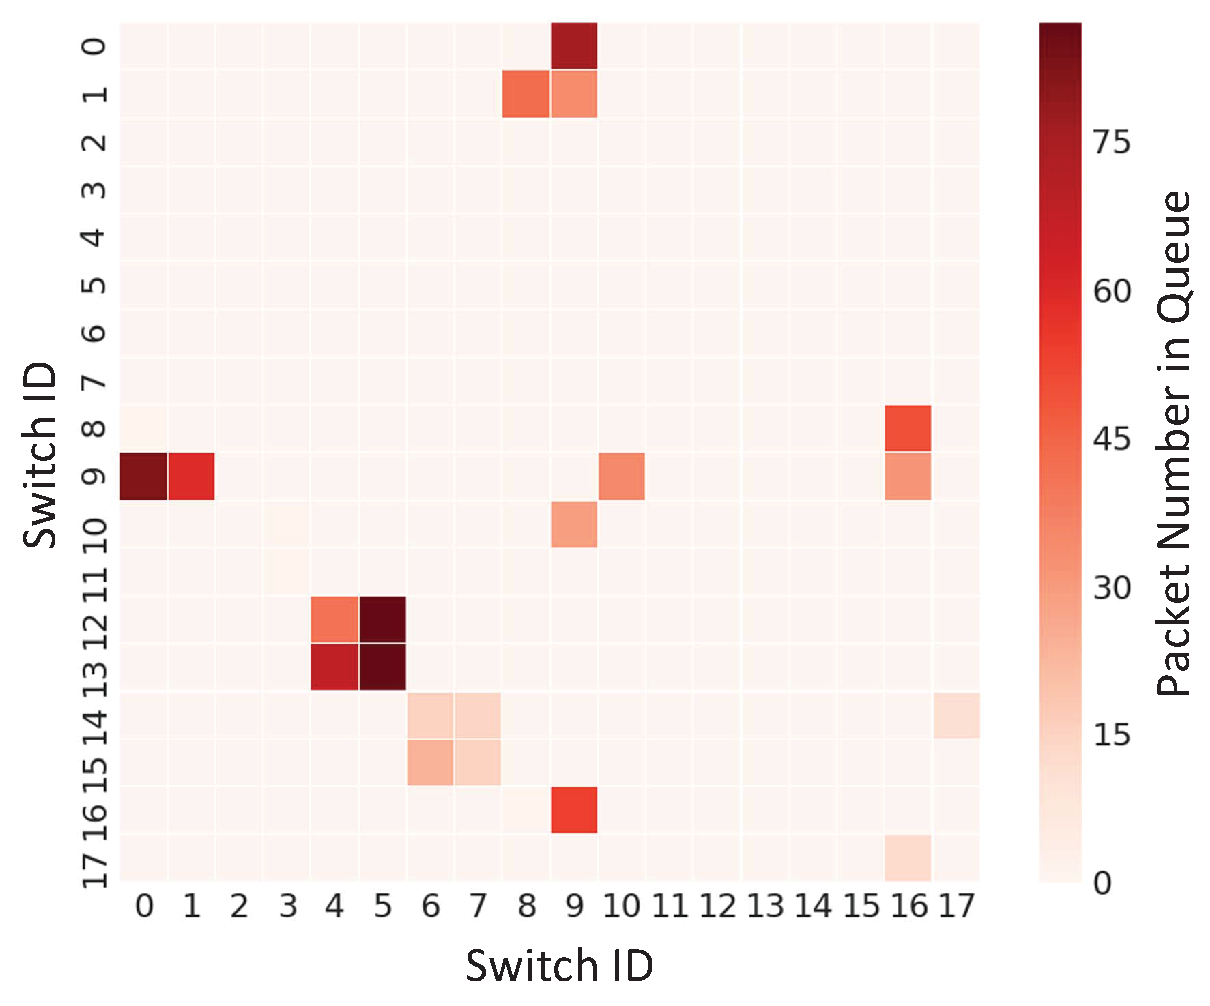
\includegraphics[width=0.22\textwidth]{figure/bitmap_low.eps}\label{fig:bitmap_low}}
\vspace{-0.1cm}
\subfigure[Network is heavily loaded.]{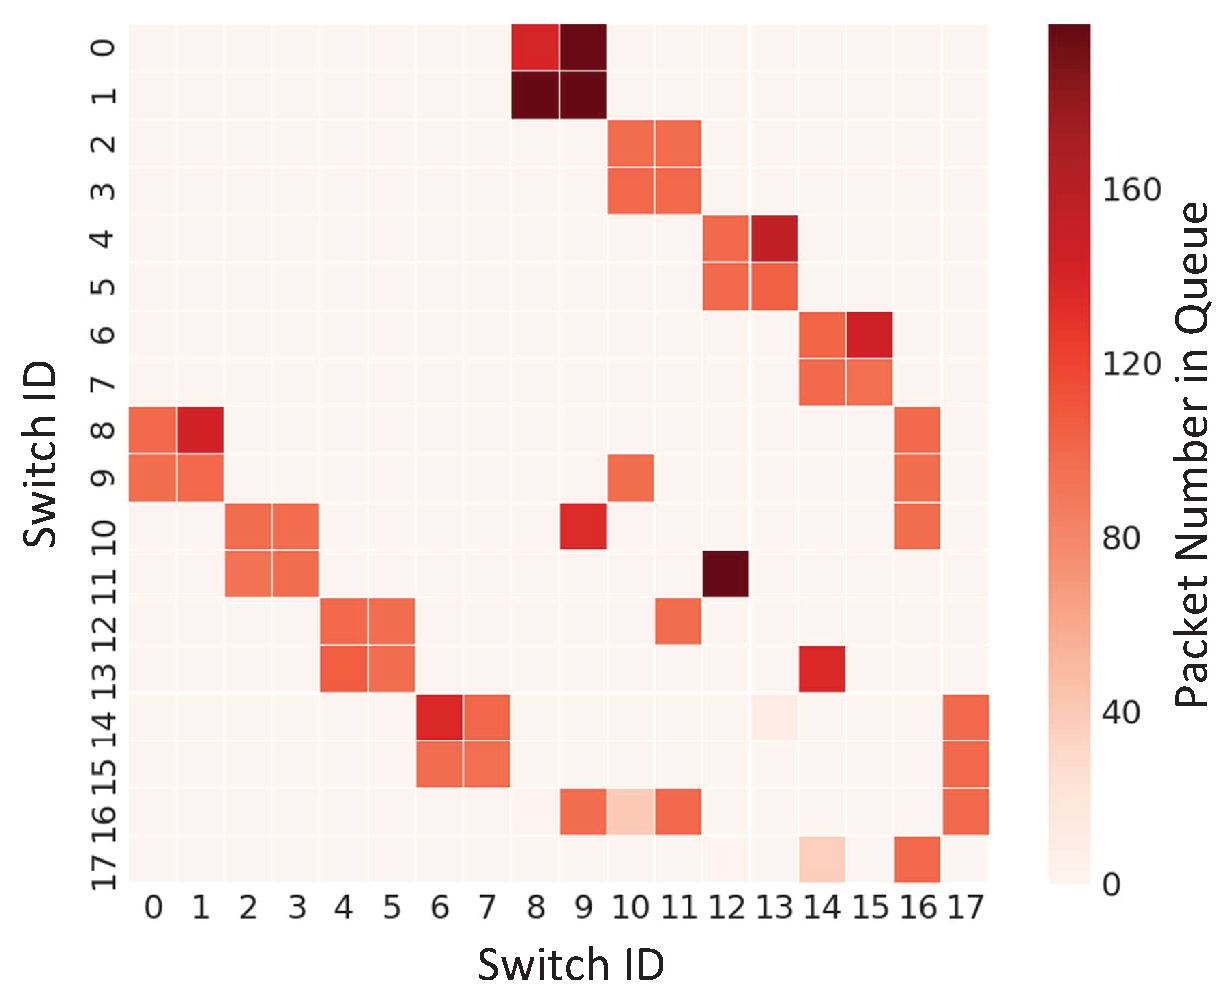
\includegraphics[width=0.22\textwidth]{figure/bitmap_high.eps}\label{fig:bitmap_high}}
\vspace{-0.1cm}
\caption{Network-wide traffic visibility as a series of ``bitmap images''.}
\label{fig:bitmap}
\vspace{-0.4cm}
\end{figure}

\subsection{Experimental Results}

\begin{figure*}[htbp]
	\vspace{-0.2cm}
\minipage{0.24\textwidth}
	\vspace{0.0cm} \includegraphics[width=\linewidth]{figure/path_num.eps}
	  \center
	  \vspace{-0.0cm}
	  \caption{Number of INT paths from DFS and Euler trail-based algorithms.}\label{fig:path_num}
	\endminipage\hfill
    	\minipage{0.24\textwidth}
					\vspace{-0.0cm} \includegraphics[width=\linewidth]{figure/fix_odd.eps}
					  \center
					  \vspace{0.0cm}
					  \caption{Number of INT paths generated under a fixed odd vertex number}\label{fig:fix_odd}
					\endminipage\hfill
	\minipage{0.24\textwidth}
                    \vspace{-0.0cm} 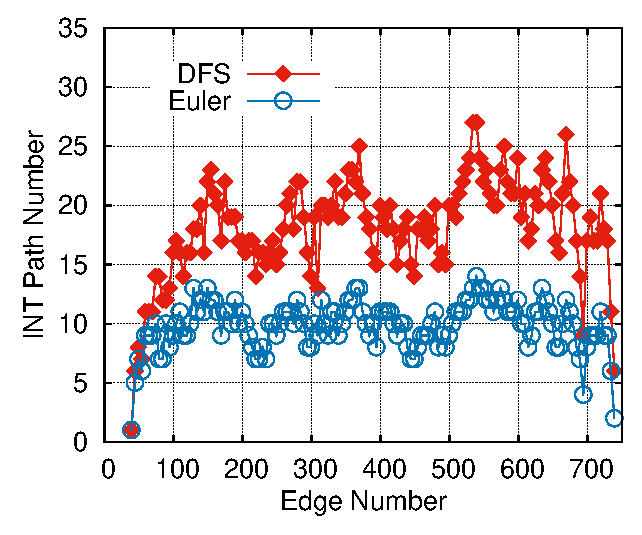
\includegraphics[width=\linewidth]{figure/fix_vertex.eps}
			  \center
			  \vspace{-0.0cm}
			  \caption{Number of INT paths generated under a fixed vertex number}\label{fig:fix_vertex}
			\endminipage\hfill
					\minipage{0.244\textwidth}
					\vspace{-0.0cm} \includegraphics[width=\linewidth]{figure/balance.eps}
					  \center
					  \vspace{0.0cm}
					  \caption{Variance of path lengths with balanced and unbalanced algorithms.}\label{fig:balance}
					\endminipage
					 
\vspace{-0.3cm}
\end{figure*}


\begin{figure*}[htbp]
	\vspace{-0.0cm}
\minipage{0.24\textwidth}
	\vspace{0.0cm} 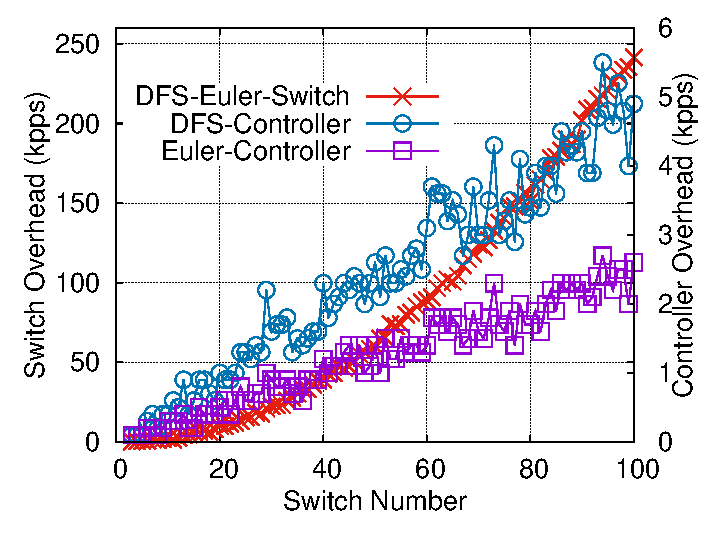
\includegraphics[width=\linewidth]{figure/overhead.eps}
	  \center
	  \vspace{-0.0cm}
	  \caption{Telemetry overhead of DFS and Euler on controller and data plane.}\label{fig:overhead}
	\endminipage\hfill
	\minipage{0.24\textwidth}
			\vspace{-0.0cm} \includegraphics[width=\linewidth]{figure/runtime.eps}
			  \center
			  \vspace{-0.0cm}
			  \caption{Execution time of DFS and Euler upon a growing network size.}\label{fig:runtime}
			\endminipage\hfill
			\minipage{0.255\textwidth}
					\vspace{-0.0cm} 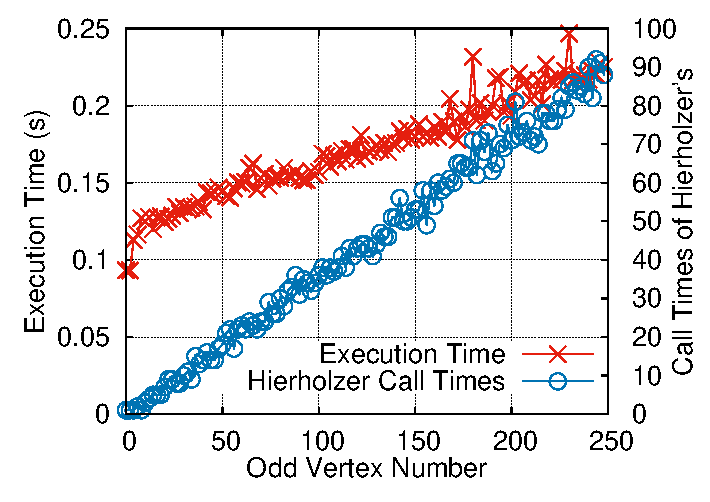
\includegraphics[width=\linewidth]{figure/odd.eps}
					  \center
					  \vspace{0.0cm}
					  \caption{Impact of odd vertex number on Euler's execution time (500 switches.)}\label{fig:odd}
					\endminipage\hfill
					\minipage{0.24\textwidth}
					\vspace{-0.0cm} 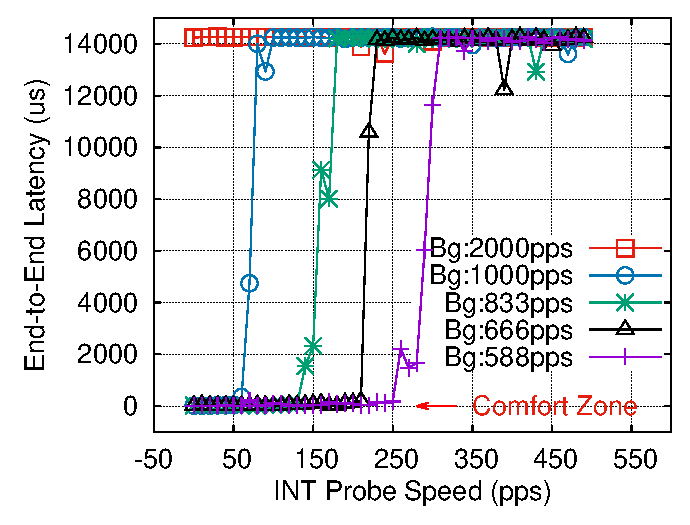
\includegraphics[width=\linewidth]{figure/impact.eps}
					  \center
					  \vspace{0.0cm}
					  \caption{Impact of telemetry granularity on system performance.}\label{fig:impact}
					\endminipage
					 
\vspace{-0.55cm}
\end{figure*}

\textbf{Number of generated INT path.}
Fig.~\ref{fig:path_num} shows the number of generated INT paths from DFS and Euler trail-based algorithms on randomly generated graphs. The path number of both DFS and Euler grow roughly linearly with the graph size while the Euler generates less INT paths than DFS under any fixed switch number. As we have mentioned, the number of paths generated from Euler is the theoretical minimum and only decided by the odd vertex number of the graph. In Fig.~\ref{fig:path_num}, since the graph is randomly created, Euler's path number grows together with the odd vertex number as the graph becomes larger. In Fig.~\ref{fig:fix_odd}, when we fix the number of odd vertices in a graph, the INT path number generated from Euler becomes a constant no matter what size the network grows into. In Fig~\ref{fig:fix_vertex}, when we fix the number of vertices to a constant (\eg, 39 in our experiment) and grow the network size by adding more edges, we can find that the path number generated from both DFS and Euler grow at the first and decline in the end. This is because adding more edges at the start makes the graph become more complex with more odd vertices while in the end, the graph finally becomes a complete graph without odd vertices (in a complete graph, every pair of distinct vertices is connected by a unique edge and each of the 39 vertices has 38 connected edges). Despite this, Euler still outperforms DFS to generate less INT paths in Fig~\ref{fig:fix_vertex}.

\textbf{Balanced vs unbalanced path generation.}
Fig~\ref{fig:balance} shows the variance of the path lengths generated from the original version of Euler and a later improved version considering path balance (\S\ref{subsec:balance}). We can figure out that by adding the heuristic for balanced path generation by rewriting \texttt{randomTrail()}, the variance of the path lengths becomes lower compared with the original Euler on randomly generated graphs.



\textbf{Telemetry overhead.}
Fig.~\ref{fig:overhead} shows the INT telemetry overhead of DFS and Euler trail-based algorithms on both the controller and the switches. The telemetry overhead on the controller is mainly caused by INT probe collection. The traffic volume of the probes forwarded to the controller is decided by the INT sending rate as well as the number of INT collectors, which is further decided by the number of INT paths generated by the algorithms. In Fig.~\ref{fig:overhead}, when the switch number is 100, DFS floods 5kpps probes to the controller while Euler only floods 2.5kpps due to the minimum generated path number. For the data plane, the telemetry overhead is measured as the total number of INT probes processed by switches per second. Since both DFS and Euler will traverse all edges of the graph, they have the same switch telemetry overhead. The switch telemetry overhead is only affected by the network size and the INT sampling granularity.

\textbf{Execution time of path planning algorithms.}
Fig.~\ref{fig:runtime} shows the execution time of DFS and Euler upon a growing network size. According to our exhaustive analysis of Euler's run-time complexity in \S\ref{subsec:theory}, Euler's execution time is larger than DFS's. Besides, Euler's execution time is more sensitive to the odd vertex number of the graph. In Fig.~\ref{fig:odd}, we find that the execution time of Euler trail-based algorithm grows roughly linearly with the odd vertex number. This result also validates our run-time complexity analysis that the subprocedures \texttt{randomTrail()}, \texttt{EulerTrail()} and \texttt{EulerCircuit()} are most frequently executed in our algorithm which are related with the odd vertex number.

\textbf{Impact of telemetry granularity.}
To achieve fine-grained network-wide telemetry, \ie, to obtain the precise real-time traffic dynamics in the network, the INT probe generation speed is expected to be as high as possible. However, this will not only lay heavy performance burden on the controller, but also occupy the limited link bandwidth, causing traffic congestion or even router buffer overflow. That is to say, there should be a limit of the telemetry granularity, constrained by controller's ability and link's capacity. Fig.~\ref{fig:impact} shows this extreme situation. In Fig.~\ref{fig:impact}, the x-axis is the INT probe generation speed at each end host and the y-axis is the end-to-end link latency along the probing path. We can figure out that when the INT probe generation speed grows, there is a sudden change of the end-to-end latency. This is because the buffer of the switches along the probing path become overflow at that time and start to drop packets. To make the experimental results more significant, we set a shallow buffer of 100 packets for each P4 switch and the buffer overflow occurs very soon. Besides, the background traffic rate also has an impact on the end-to-end latency of the probe packets. For INT-path deployment in real-world networks, we recommend to properly arrange the telemetry granularity into the ``comfort zone'' in Fig.~\ref{fig:impact}, considering the switch buffer size configuration and the background traffic rate.
%需要讲队列长度比较短,几百,一会儿就满了,导致最大时延比较恒定



\textbf{Network-wide telemetry in DC networks.}
In the previous sections, we discuss the performance of Euler trail-based algorithm on randomly generated graphs. Here, we investigate its performance in today's data center networks. Designing for better load balancing, classic data center network topologies are symmetric and have several multi-path topology patterns. Fig.~\ref{fig:dc} shows two classic DC network topologies: FatTree and LeafSpine. We find that the odd vertex number in both topologies are very predictable depending on the scale of the networks. For example, in FatTree, there are three layers of switch nodes, and the layer 1 and layer 3 do not have odd vertices no matter what the scale of the network. However, in layer 2, the number of the odd vertices regularly changes depending on the size of the network. LeafSpine shows the similar property. This property is very helpful when we design DC networks with In-band network-wide telemetry features. If the DC network topology has an even number of basic units (as shown in Fig~\ref{fig:dc}), at best, we can use one INT telemetry path to cover the entire network. If it has an odd number $\ie, k$ of units, we have to plan $k$ telemetry paths for the full network coverage. Fig.~\ref{fig:topo} shows the comparison between DFS and Euler on DC network topologies. We can find the symmetric topology of DC networks even makes DFS output predicable! However, Euler still outperforms DFS in either DC topology.

\begin{figure}
\centering
\epsfig{file=figure/dc.eps, scale=0.45}
\vspace{-0.3cm}
\caption{Two classic data center network topologies.}
\label{fig:dc}
\vspace{-0.4cm}
\end{figure}



\begin{figure}[t]
\vspace{-0.0in}
\centering
\subfigure[FatTree topology.]{\includegraphics[width=0.23\textwidth]{figure/fat_tree.eps}\label{fig:fat_tree}}
\vspace{-0.15cm}
\subfigure[LeafSpine topology.]{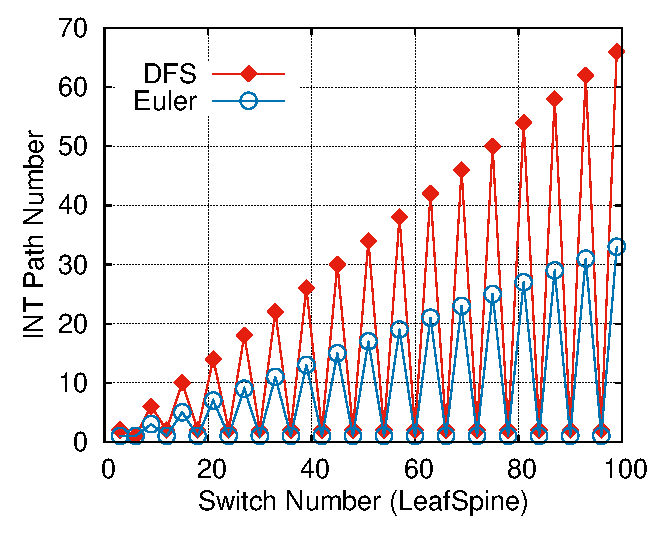
\includegraphics[width=0.23\textwidth]{figure/leaf_spine.eps}\label{fig:leaf_spine}}
\vspace{-0.15cm}
\caption{Euler outperforms DFS with classic data center network topologies.}
\label{fig:topo}
\vspace{-0.4cm}
\end{figure}